%% This is file `elsarticle-template-1-num.tex',
%% %% Copyright 2009 Elsevier Ltd
%%
%% This file is part of the 'Elsarticle Bundle'.
%% ---------------------------------------------
%%
%% It may be distributed under the conditions of the LaTeX Project Public
%% License, either version 1.2 of this license or (at your option) any
%% later version.  The latest version of this license is in
%%    http://www.latex-project.org/lppl.txt
%% and version 1.2 or later is part of all distributions of LaTeX
%% version 1999/12/01 or later.
%%
%% The list of all files belonging to the 'Elsarticle Bundle' is
%% given in the file `manifest.txt'.
%%
%% Template article for Elsevier's document class `elsarticle'
%% with numbered style bibliographic references
%%
%% $Id: elsarticle-template-1-num.tex 149 2009-10-08 05:01:15Z rishi $
%% $URL: http://lenova.river-valley.com/svn/elsbst/trunk/elsarticle-template-1-num.tex $
%%

%\documentclass[]{article}
\documentclass[preprint,3p,12pt]{elsarticle}
%\documentclass[final,5p,times,twocolumn]{elsarticle}

%% Use the option review to obtain double line spacing
%% \documentclass[preprint,review,12pt]{elsarticle}

%% Use the options 1p,twocolumn; 3p; 3p,twocolumn; 5p; or 5p,twocolumn
%% for a journal layout:
%% \documentclass[final,1p,times]{elsarticle}
%% \documentclass[final,1p,times,twocolumn]{elsarticle}
%% \documentclass[final,3p,times]{elsarticle}
%% \documentclass[final,3p,times,twocolumn]{elsarticle}
%% \documentclass[final,5p,times]{elsarticle}
%% \documentclass[final,5p,times,twocolumn]{elsarticle}

%% if you use PostScript figures in your article
%% use the graphics package for simple commands
%% \usepackage{graphics}
%% or use the graphicx package for more complicated commands
%% \usepackage{graphicx}
%% or use the epsfig package if you prefer to use the old commands
%% \usepackage{epsfig}

%% The amssymb package provides various useful mathematical symbols
\usepackage{amssymb}
\usepackage{wrapfig}
\usepackage{lipsum}

\usepackage{tikz}
\usepackage{mathdots}
\usetikzlibrary{shapes, arrows}

\usepackage{graphicx}
\graphicspath{ {./graphics/} }


%% Styles for proximity flow chart
\tikzstyle{ccell} = [rectangle, draw, fill=red!20, minimum width=3em, text centered, minimum height=3em]
\tikzstyle{dcell} = [rectangle, draw, fill=brown!20, minimum width=3em, text centered, minimum height=3em]
\tikzstyle{gcell} = [rectangle, draw, fill=yellow!20, minimum width=3em, text centered, minimum height=3em]
\tikzstyle{fcell} = [rectangle, draw, fill=green!20, minimum width=3em, text centered, minimum height=3em]
\tikzstyle{ucell} = [rectangle, draw, fill=white!20, minimum width=3em, text centered, minimum height=3em]
\tikzstyle{line} = [draw, -latex']


\journal{University of Guelph; CIS*4780}

\begin{document}

\begin{frontmatter}

\title{Two Dimensional Intelligent Character Recognition}

%% use optional labels to link authors explicitly to addresses:
%% \author[label1,label2]{<author name>}
%% \address[label1]{<address>}
%% \address[label2]{<address>}

%\author{Ryan Pattison & Douglas Anderson & Oliver Cook}
\author[ryan,doug,oliver]{Ryan Pattison, Douglas Anderson, and Oliver Cook}
\address[ryan]{ryan.m.pattison@gmail.com}
\address[doug]{dander01@uoguelph.ca}
\address[oliver]{cooko@uoguelph.ca}


\begin{abstract}

For quite some time computer vision has been used to extract characters from
images in order to gain knowledge from text. In recent years many of the
techniques for recognizing characters has been based on machine learning.

\end{abstract}

\begin{keyword}
% keywords here, in the form: keyword \sep keyword
Machine Learning \sep
Data Mining \sep
Computer Vision \sep
Intelligent Character Recognition

%% MSC codes here, in the form: \MSC code \sep code
%% or \MSC[2008] code \sep code (2000 is the default)

\end{keyword}

\end{frontmatter}


%% main text
\section{Introduction}
\label{intro}

The problem of Intelligent Character Recognition (ICR) in Artificial
Intelligence and Machine Learning has received much attention in past years.
This field of study has focused on the classification of \emph{handwritten}  or
\emph{typewritten} letters and numbers.  The novelty of this project will be in
the development of an algorithm which recognizes characters, or more generally
symbols, arranged to form words in \emph{two} dimensions. The practical
application proposed here will be the development of an algorithm for
recognizing hand drawn cartography. To this end, we have defined a small set of
symbols to represent various terrains: grass, mountains, bodies of water, and
more. Each symbol will be drawn into a single cell on a standard sheet of grid
paper and scanned into a computer. Using the scanned images, the proposed
algorithm will learn to recognize the symbols cell by cell as well as in the
context of the information in the surrounding cells. In order to demonstrate
the utility of such an algorithm, we propose an application which will read a
hand drawn map and produce a computer generated image showing the same map.

\section{Process}
\label{process}

\subsection{Overview}
\label{process:overview}

\begin{figure}
\begin{center}
\includegraphics[width=2in]{PokemonPalletTown.png}
\end{center}
\caption{Pallet Town map from Pok\'{e}mon} 
\end{figure}


We have created 6 symbols to be used to recreate maps for a popular video game
Pok\'{e}mon to ensure that our data set is sampled from some well defined distribution.


\begin{tabular}{llll}
Water & \includegraphics[width=.5in]{water.png} &
Grass & \includegraphics[width=.5in]{grass.png} \\
Rock & \includegraphics[width=.5in]{rocks.png} &
Tree & \includegraphics[width=.5in]{tree.png} \\
Dirt & \includegraphics[width=.5in]{dirt.png} &
Sand & \includegraphics[width=.5in]{sand.png} \\
\end{tabular}

\subsection{Preprocessing}
\label{process:preprocessing}

For all of our analysis we pre-process colour images images into black and white
images. To do this we first remove the blue grid lines from the image and
replace them with white. We then remove all colour information from the image
and resize it such that every cell of the grid is 75 pixels by 75 pixels.

\begin{figure}[h]
    \begin{center}
    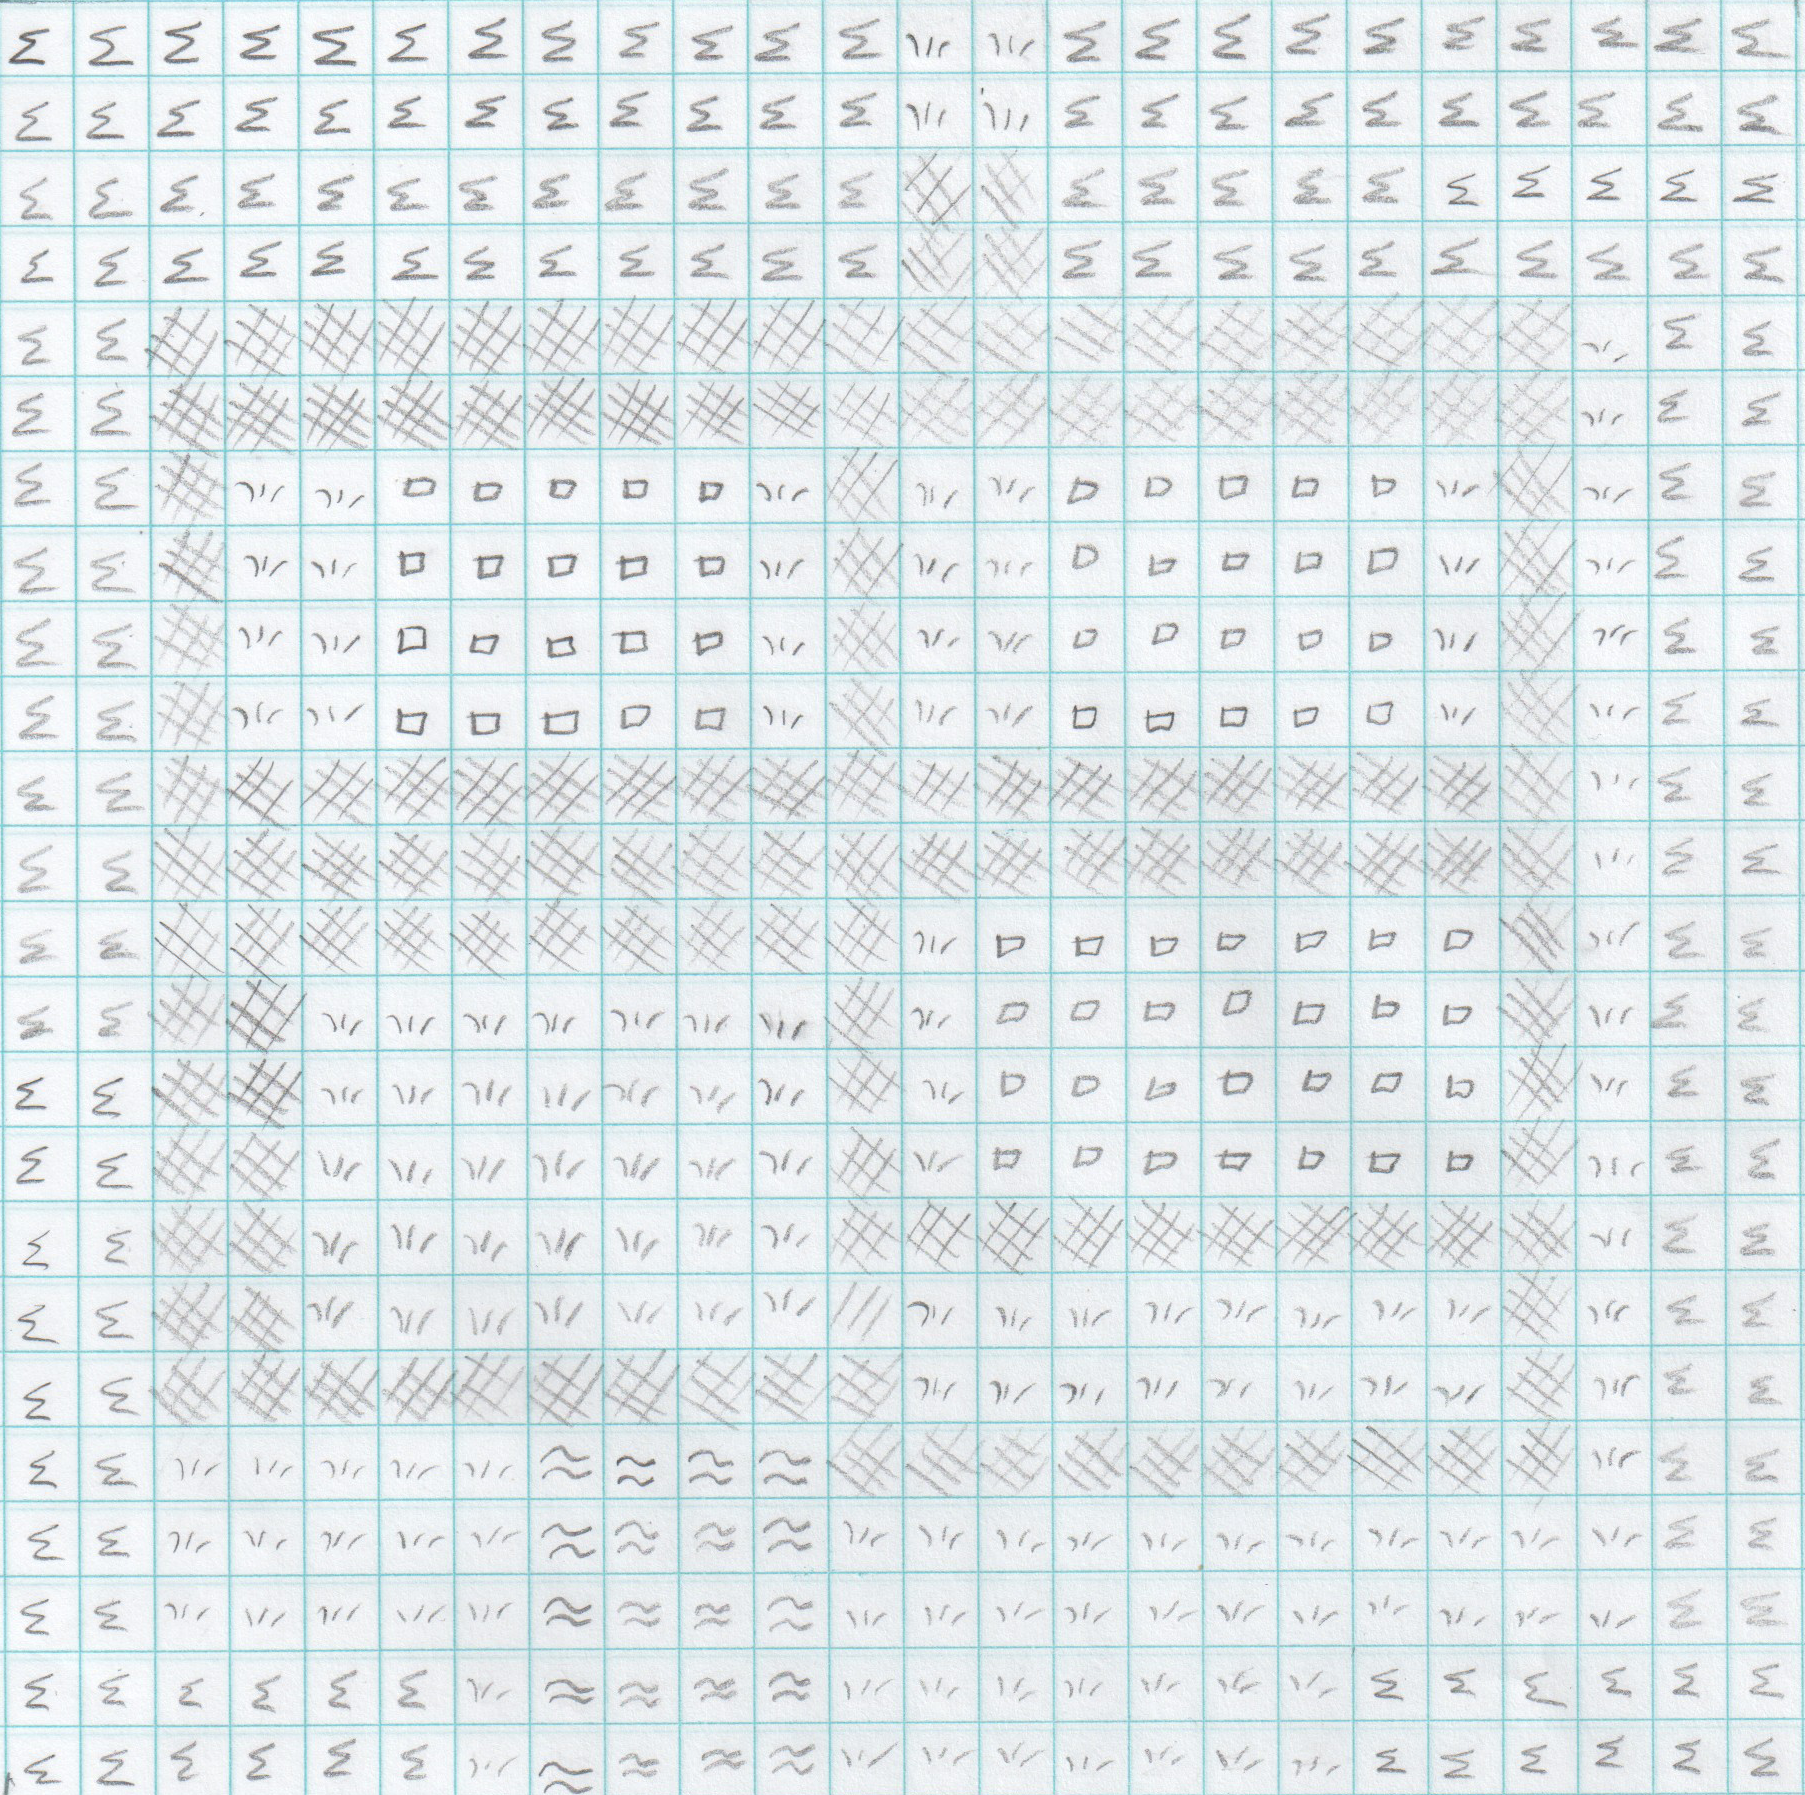
\includegraphics[width=7.5cm, height=7.5cm]{preprocessing-initial}
    \includegraphics[width=7.5cm, height=7.5cm]{preprocessing-final}

    \caption{Image before preprocessing and image after preprocessing. Notice
        that the contrast has increased and the blue lines have been partially
        removed}

    \end{center}
\end{figure}

\subsection{Feature-Based Approach}
\label{process:featurebased}

The Feature-Based approach used here applies convolution filters to the cell images and then
gathers statistics based on the distribution of black pixels in each of the $x$ and $y$ dimensions.
A convolution filter is matrix of coefficients of odd size. Below is a convolution filter for a
mean blur.

\[
F_{blur} = \left[
\begin{array}{ccc}
1/16 & 2/16 & 1/16 \\
2/16 & 4/16 & 2/16 \\
1/16 & 2/16 & 1/16
\end{array}\right]
\]


If we consider a single cell of the grid, a portion of the image with one symbol in it, as a matrix
of luminance values like so:

\begin{figure}
\[
\begin{array}{lcr}
\begin{array}{ccccc}
\ddots & \vdots & \vdots & \vdots & \iddots \\
\ldots & 64 & 64 & 32 & \ldots \\
\ldots & 32 & \fbox{32} & 128 & \ldots \\
\ldots & 32 & 16 & 32 & \ldots \\
\iddots & \vdots & \vdots & \vdots & \ddots \\
\end{array} &
\begin{array}{c}
64F_{11} + 64F_{12} + 32F_{13} \\
+ 32F_{21} + 32F_{22} + 128F_{23} \\
+ 32F_{31} + 16F_{32} + 32F_{32} \\
\end{array} &
\begin{array}{ccccc}
\ddots & \vdots & \iddots \\
\ldots &  48  & \ldots \\
\iddots & \vdots & \ddots \\
\end{array}
\end{array}
\]
\end{figure}

The filtering process repeats for each pixel until all pixels have been replaced.
The resulting image has the luminance matrix $A$.

\[
A =
\left [
    \begin{array}{r r r r}
        a_{00} & a_{10} & \cdots & a_{n0} \\
        a_{01} & a_{11} & \cdots & a_{n1}\\
        \vdots  & \vdots  & \ddots & \vdots\\
        a_{0m} & a_{1m} & \cdots & a_{nm}\\
    \end{array}
\right ]
\]

We define $x$ and $y$ to be the row and column sum functions.

\begin{equation}
x(i) = \sum_{j}{A_{i,j}} \quad
y(j) = \sum_{i}{A_{i,j}}
\end{equation}

Next we record $\mu_x, \mu_y, \sigma_x, \sigma_y$ as the feature set for this filter.


\subsection{Gold Comparison Approach}


\begin{figure}[h]
\includegraphics{building-mean}
\includegraphics{dirt-mean}
\includegraphics{forest-mean}
\includegraphics{grass-mean}
\includegraphics{water-mean}
\includegraphics{rocks-mean}

\caption{The gold images created as the mean image of all examples of each symbol. In order we have symbols reprenting buildings, dirt, forest, grass, water, and rocks.}

\end{figure}

Similar to the Feature-based approach we define $x$ and $y$ to be the row and column sums and calculate the mean and standard deviation.
To get the symbols to overlap we apply a linear transformation to each pixel using the statistics gathered in each dimension.
\begin{equation} \label{eq:gold}
x^{\prime} = (x - \mu^{B}_{x}) \, \frac{\sigma^{G}_{x}}{\sigma^{C}_{x}} + \mu^{G}_{x} \quad
y^{\prime} = (y - \mu^{B}_{y}) \, \frac{\sigma^{G}_{y}}{\sigma^{C}_{y}} + \mu^{G}_{y}
\end{equation}

We then compare the overlapping image $A$ to the gold standard image $G$ by taking the sum of the squared difference at each pixel position.
This gives us an error measure which we record for each class $k$.

\[
\xi_{k}(A) = \sum_{i}\sum_{j}{(A_{ij} - G_{kij})^{2}}
\]

The result is a vector of size $k$, the number of classes, with an error measure for the comparison
against the corresponding class. We then input this vector into WEKA along with the correct answer
for training purposes. We used a J48 decision tree with 10-fold validation.

\subsection{Proximity Approach}
\label{process:proximity}

We want to classify the symbol $x$, and we do this by first calculating the
probability that $x$ belongs to each class, $P(X)\quad X_i = P(x\!\in\! C_i)$.
The proximity classifier is given the class of each symbol in the
cardinal directions: north, south, east, and west. Using this information,
we restrict the probability calculation to only consider the subspace
where a symbol has the given classes neighbouring it. Such a restriction is
the conditional probability:
\[
P(X) = P(X|\,N\!=\!c_1,\,E\!=\!c_2,\,S\!=\!c_3,\,W\!=\!c_4)
\]
In calculating probabilities, we can only approximate them using relative
frequencies collected from our sample data. For a set of $k$ classes, there are $k^4$ possible combinations of neighbouring
cells and too many of these combinations occur rarely in our dataset to make
confident approximations of the true probabilities. To resolve this, we assume that
the conditional probabilities are independent in each direction. Under this
assumption, the calculation becomes much more reasonable for our small data set
since there are only $4k$ possible combinations. Our resulting calculation becomes:

\begin{equation} \label{eq:prox}
P(X) \approx P(X|\,N\!=\!c_1)P(X|\,S\!=\!c_2)P(X|\,E\!=\!c_3)P(X|\,W\!=\!c_4)
\end{equation}

From the definition of conditional probability we have that for some class $c$ in
the direction $D$:
\[ P(X|\,D\!=\!c) = \frac{P(X \cap D\!=\!c)}{P(D=c)} \]
To calculate each of the conditional probabilities,
we compute a table from the samples which records $P(X\cap D\!=\!c)$ and $P(D\!=\!c)$ for each class and direction.
We use the table to calculate the relative conditional frequencies and, under the assumption
of independence, we approximate $P(X)$ using equation ~\ref{eq:prox}.

Having the probability vector $P(X)$ under the assumption of independence, we create an input file for WEKA.
This file includes the probability vector, the neighbouring classes, and the class of the
symbol being classified for training. WEKA creates a decision tree which is used to reduce the error in the probability
calculation introduced under the assumption of independence.

\begin{figure}[h]
\begin{center}
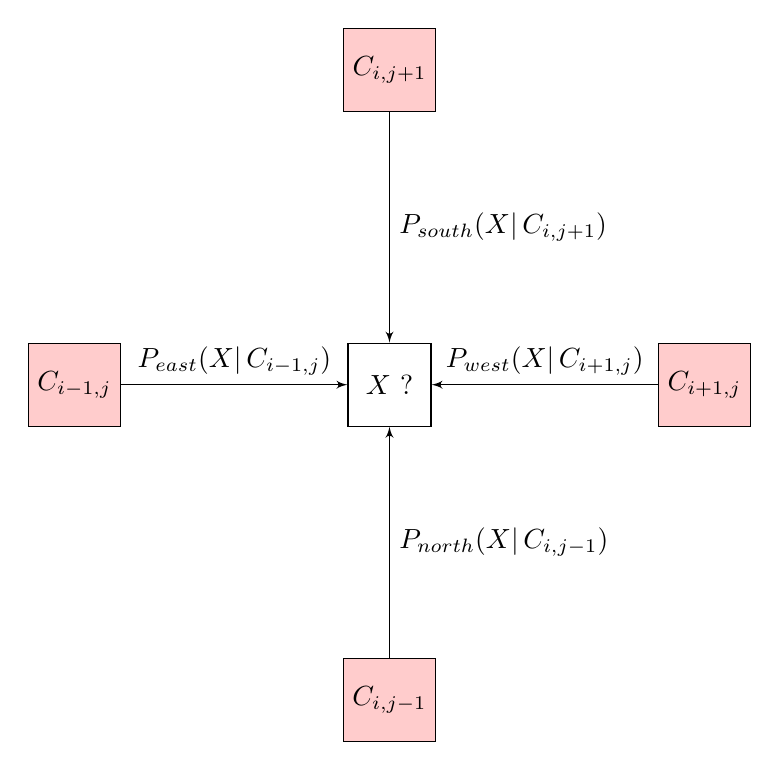
\begin{tikzpicture}[node distance = 4 cm, auto]
    \node[ccell](top){$C_{i,j+1}$};
    \node[ucell, below of=top](center){$X$~?};
    \node[ccell, left of=center](left){$C_{i-1,j}$};
    \node[ccell, right of=center](right){$C_{i+1,j}$};
    \node[ccell, below of=center](bottom){$C_{i,j-1}$};

    \path[line] (top)   -- node[right] {$P_{south}(X | \, C_{i,j+1})$} (center);

    \path[line] (left)  -- node[above] {$P_{east}(X | \, C_{i-1,j})$} (center);
    \path[line] (right) -- node[above] {$P_{west}(X | \, C_{i+1,j})$} (center);
    \path[line] (bottom) -- node[right] {$P_{north}(X | \, C_{i,j-1})$} (center);
\end{tikzpicture}
\end{center}
\caption{This figure describes the probability of class $X$ neighbouring cells $C_{i,j}$}
\end{figure}


Let $V_{d}$ be a vector of probabilities, where $n$ is the number of classes,
$d$ is a direction.

\begin{equation}
V_{d} = \left(P_{d}{(X_{1} | \, C_{d})}, P_{d}{(X_{2} | \, C_{d}),\; \ldots \; , P_{d}{(X_{n} | \, C_{d}})}\right)
\end{equation}

To determine the probability of a cell belonging in a particular class, we assume independence
so that we can multiply the vectors of all directions together using the element-wise product.

\begin{equation}
C_{centre} = V_{north} \circ V_{east} \circ V_{south} \circ V_{west}
\end{equation}

This new vector $C_{centre}$ contains $n$ probabilities that this cell should be
classified as a particular class. One approach to classifying the unknown symbol
would be to choose the class corresponding to the maximum probability in $C_{centre}$.

An example of this process can be seen with the following situation. Suppose
that the training set has the following characteristics:

\begin{table}[h]
\small
\begin{center}
\begin{tabular}{ l | r r r r r r }
              & $c_{B}$& $c_{D}$& $c_{EDGE}$& $c_{F}$& $c_{G}$& $c_{W}$ \\ 
              \hline
    north     & 0      & 0.1558 & 0.0519    & 0.0519 & 0.7403 & 0.0325\\
    east      & 0.0779 & 0.0974 & 0         & 0.1493 & 0.6428 & 0\\
    south     & 0      & 0.2403 & 0.0130    & 0.0065 & 0.7403 & 0\\
    west      & 0.0519 & 0.2273 & 0         & 0.0519 & 0.6428 & 0.0260\\
\end{tabular}
\caption{The probability of the class of neighbours in each direction for a
    grass cell from the map that we created entitled PalletTown} 
\end{center}
\end{table}

\begin{figure}[h]
\begin{center}
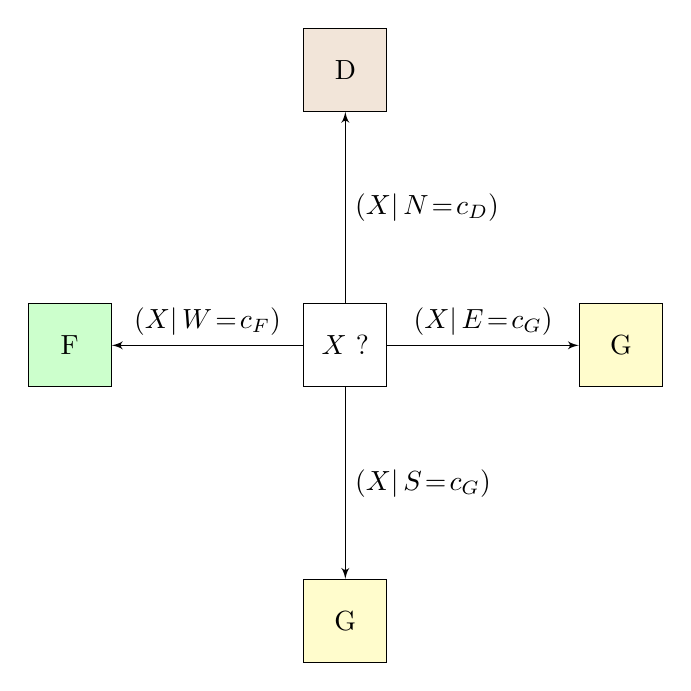
\begin{tikzpicture}[node distance = 3.5 cm, auto]
    \node[dcell](top){D};
    \node[ucell, below of=top](center){$X$~?};
    \node[fcell, left of=center](left){F};
    \node[gcell, right of=center](right){G};
    \node[gcell, below of=center](bottom){G};

    \path[line] (center)   -- node[right] {$(X|\,N\!=\!c_{D})$} (top);
    \path[line] (center)   -- node[above] {$(X|\,W\!=\!c_{F})$} (left);
    \path[line] (center)   -- node[above] {$(X|\,E\!=\!c_{G})$} (right);
    \path[line] (center)   -- node[right] {$(X|\,S\!=\!c_{G})$} (bottom);
\end{tikzpicture}
\end{center}
\caption{This situation includes a grass to the south and east, a dirt to the
    north and a forest to the west. It is similar to cell 2,19 in pallet town
    (when indexed from zero at the top left)}
\end{figure}

\subsection{Classifier Training}
\label{process:training}
Training was done using WEKA and 10-fold cross validation.
the proximity classifier was tested on a map it had never seen in training.

\section{Results}
\label{results}

\begin{tabular}{lllrrr}
Algorithm & Samples & Feature Set & Success & Features & Tree nodes \\\hline
Feature-Based & 9888 & Single Filter &  76.32 & 32  & ? \\
Feature-Based & 9888 & No Spatial &  80.64 & 205 & ? \\
Feature-Based & 9888 & Spatial &  82.47 & 207 & ? \\
Proximity & 13200 & Surrounding & 93.78 & 11 & ? \\ 
Gold Comparison & 225 & probabilities & 70.40 & 7 & ? \\
Gold Comparison & 225 & probabilities & 83.33 & 7 & ? \\
\end{tabular}

\section{Conclusions}
\label{conclusions}

Each of our classification methods each have their own strengths and
weaknesses.  The \textbf{Feature-Based method} is able to recognize arbitrary
features but requires intended representations of each of the maps during
training. \textbf{Proximity method} works extremely well with the set of maps
we chose because they adhere to patterns. However to detect these patterns in a
data set the proximity classifier needs a relatively accurate representation of
the map. This method has the added benift of haveing it's output be the same as
it's input.  The \textbf{Gold Comparison} method is able to classify symbols
fairly well without intended representations of the map. However this method
requires gold images as input and the number of features in the output
generated is dependent on the number of gold images.

We believe that for the best results the methods should be used in conjunction.
For example using the gold comparison method we could generate a decent
representation of the map which could then be cleaned up by the Proximity
method.


\section{Further Work}
\label{further work}
Future work may include combining the proximity classifier with the gold 
comparison classifier to improve accuracy. 

Feature based classification may see improvement from considering other
transformations of the pixels when calculating statistics, such as distance
from the centre.

Non mean golds

Regions with the feature extraction method

\section{References}
\label{references}
Pallet Town, Pokemon FireRed [screenshot]. Retreived from http://strategywiki.org/wiki/Pok%C3%A9mon_FireRed_and_LeafGreen/Pallet_Town

%% The Appendices part is started with the command \appendix;
%% appendix sections are then done as normal sections
%% \appendix

%% \section{}
%% \label{}

%% References
%%
%% Following citation commands can be used in the body text:
%% Usage of \cite is as follows:
%%   \cite{key}          ==>>  [#]
%%   \cite[chap. 2]{key} ==>>  [#, chap. 2]
%%   \citet{key}         ==>>  Author [#]

%% References with bibTeX database:

\bibliographystyle{plain}
\bibliography{refs}

%% Authors are advised to submit their bibtex database files. They are
%% requested to list a bibtex style file in the manuscript if they do
%% not want to use model1-num-names.bst.

%% References without bibTeX database:

% \begin{thebibliography}{00}

%% \bibitem must have the following form:
%%   \bibitem{key}...
%%

% \bibitem{}

% \end{thebibliography}

\end{document}

